\documentclass[11pt]{article}
\usepackage[margin=1in]{geometry}          
\usepackage{graphicx}
\usepackage{amsthm, amsmath, amssymb}
\usepackage{setspace}\onehalfspacing
\usepackage[loose,nice]{units} %replace "nice" by "ugly" for units in upright fractions
 \usepackage[UTF8, heading = false, scheme = plain]{ctex}
 \usepackage{hyperref}
 \usepackage{color}
\usepackage[normalem]{ulem}
\usepackage{url}
\usepackage[dvipsnames]{xcolor}


\DeclareUrlCommand\ULurl{%
  \renewcommand\UrlFont{\ttfamily\color{blue}}%
  \renewcommand\UrlLeft{\uline\bgroup}%
  \renewcommand\UrlRight{\egroup}}
 
\title{阅读理解实验阶段性总结}
\author{徐俊}
\date{2016年12月}


 
\begin{document}
\maketitle
\tableofcontents

\section{摘要}
阅读理解任务从七月底开始以来,至今已经快五个月,在此梳理一下开始直接的实验思路和进展。时间上来看,从八月到九月中旬,调研并达到baseline的效果;九月下旬到十月下旬针对数据和模型进行分析,在进行多项改进NN模型未果之后,大方向选择在log-linear的框架下融入经典NLP特征以及NN特征;十一月至今,大方向调整为如何利用经典NLP特征来提升任务。出于简洁直观考虑,本文按照实验类别(纯粹的模型增强实验、在log-linear框架下融入经典特征以及在NN框架下融入经典特征)分别介绍。

\section{任务概述}
参见文章《两种阅读理解模型框架的概要介绍》。两个模型框架见Figure~\ref{fig:1}和Figure~\ref{fig:2}。

\begin{figure}[htbp]
\centering
\begin{minipage}[t]{0.45\textwidth}
\centering
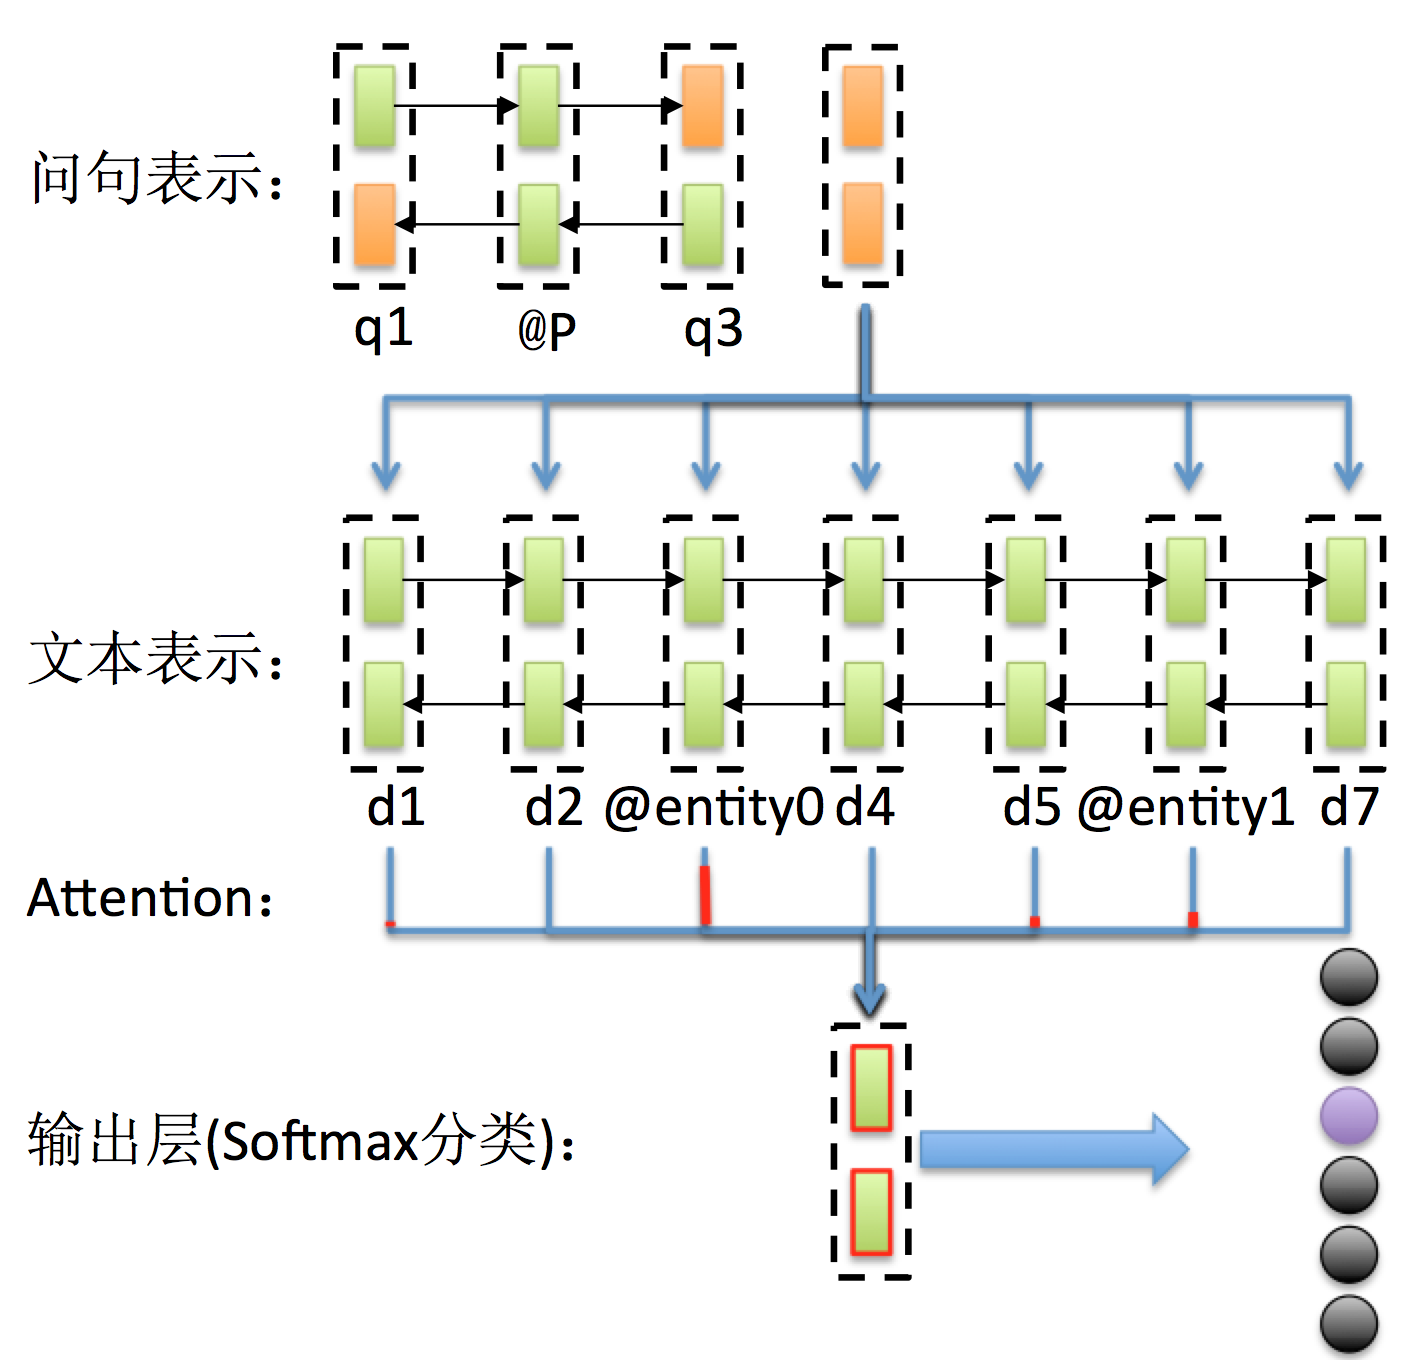
\includegraphics[width=70mm]{picture/attentionreader.png}
\caption{Attention Reader}
\label{fig:1}
\end{minipage}
\begin{minipage}[t]{0.45\textwidth}
\centering
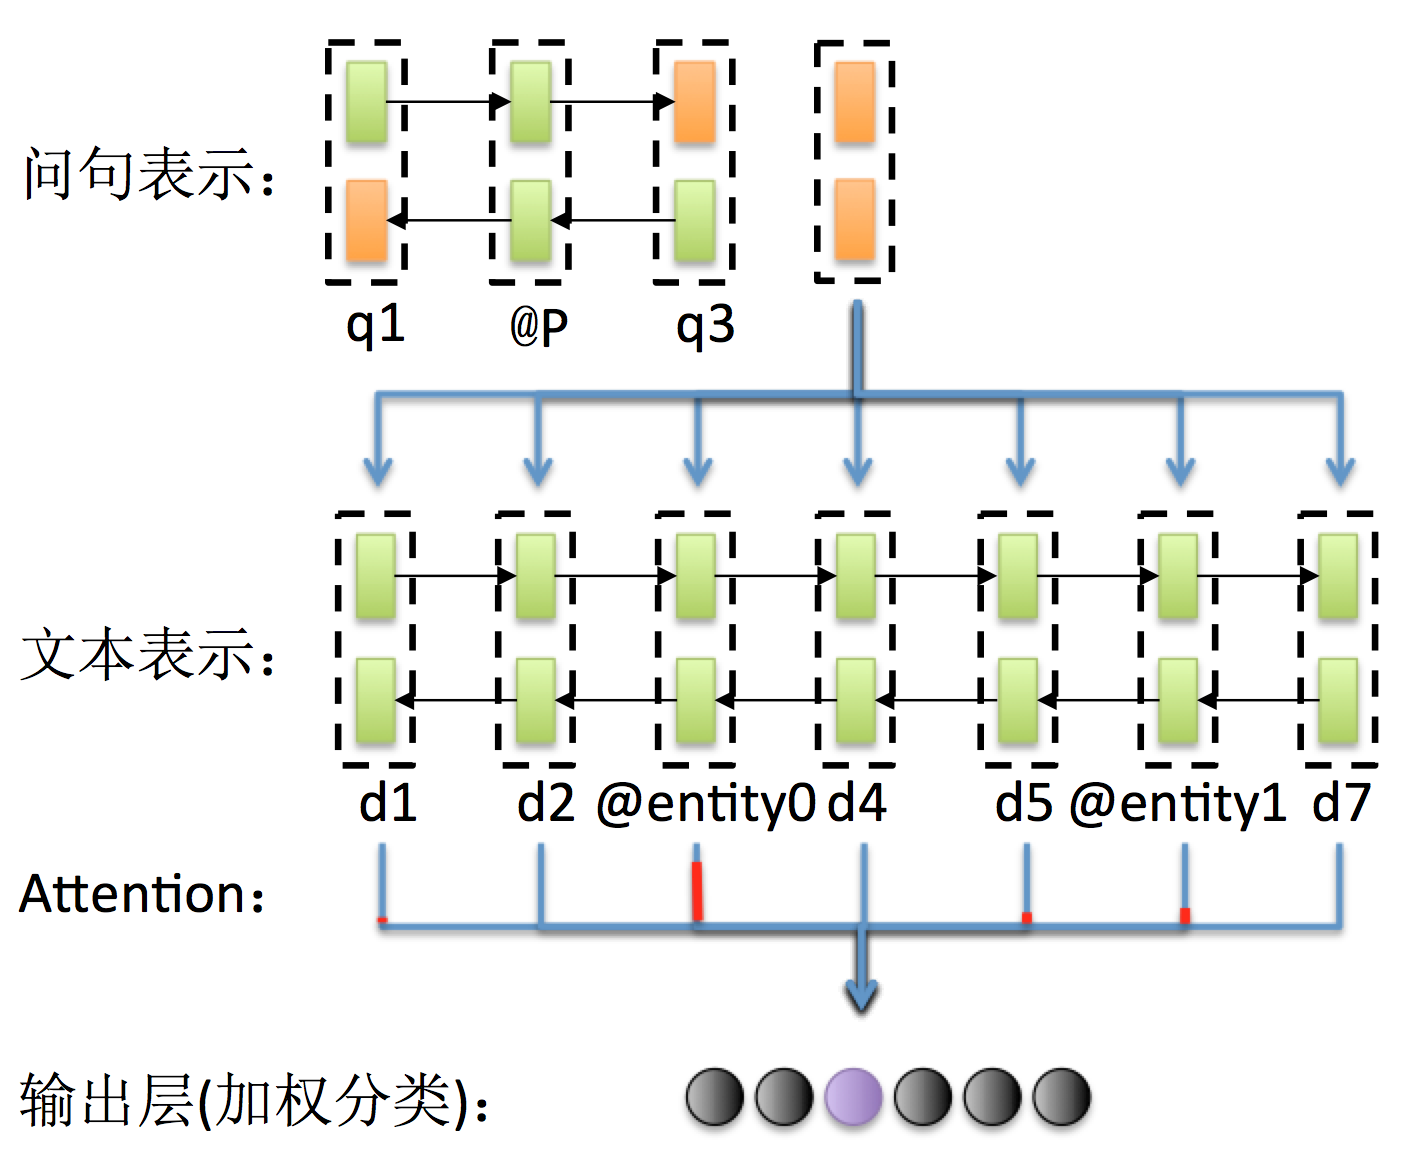
\includegraphics[width=70mm]{picture/attensumreader.png}
\caption{Attention-Sum Reader}
\label{fig:2}
\end{minipage}
\end{figure}

\section{模型增强实验}
这部分实验包括所有不涉及融入新特征的NN实验。主要分为两个大的类型:更加重视局部信息以及Attention Reader 同Attensum Reader的融合模型(Attention-Attensum Reader)。
\subsection{更加重视局部信息}
\begin{enumerate}
    \item {\bf 动机}:分析负例数据的时候发现,目标词很多时候并不是通常意义上的句子核心实体。比如问句是“探险家怎么怎样,然后乘坐帆船,从@placeholder抵达@entity1,……”,在这样的句子中目标词很难通过问句来刻画,故而想到更多的利用目标词周围信息来提升性能;
    \item  {\bf 做法}: 做法一只用目标词前后各三个词,作为“问句”,其他不变;做法二是仅利用@placeholder处的隐层状态作为问句表示;做法三是将原问句的表示同做法一中“新问句”的表示做拼接,作为问句表示;做法四是将原问句表示同做法二获得的表示做拼接,共同作为最终的问句表示;
    \item  {\bf  结果}:当时attentive reader baseline性能在71\%,而这四组模型的结果(未经严格调参的情况下)性能均没有超过70\%;
    \item  {\bf  结论以及后续}:这种做法并没有显著提升,而随着attentive reader baseline调整到72.6\%,这一部分的实验并没有继续下去,原因是感觉这个方向较为不可行;
\end{enumerate}

\subsection{Attention-Attensum Reader}
\begin{figure}[htbp]
\begin{center}
	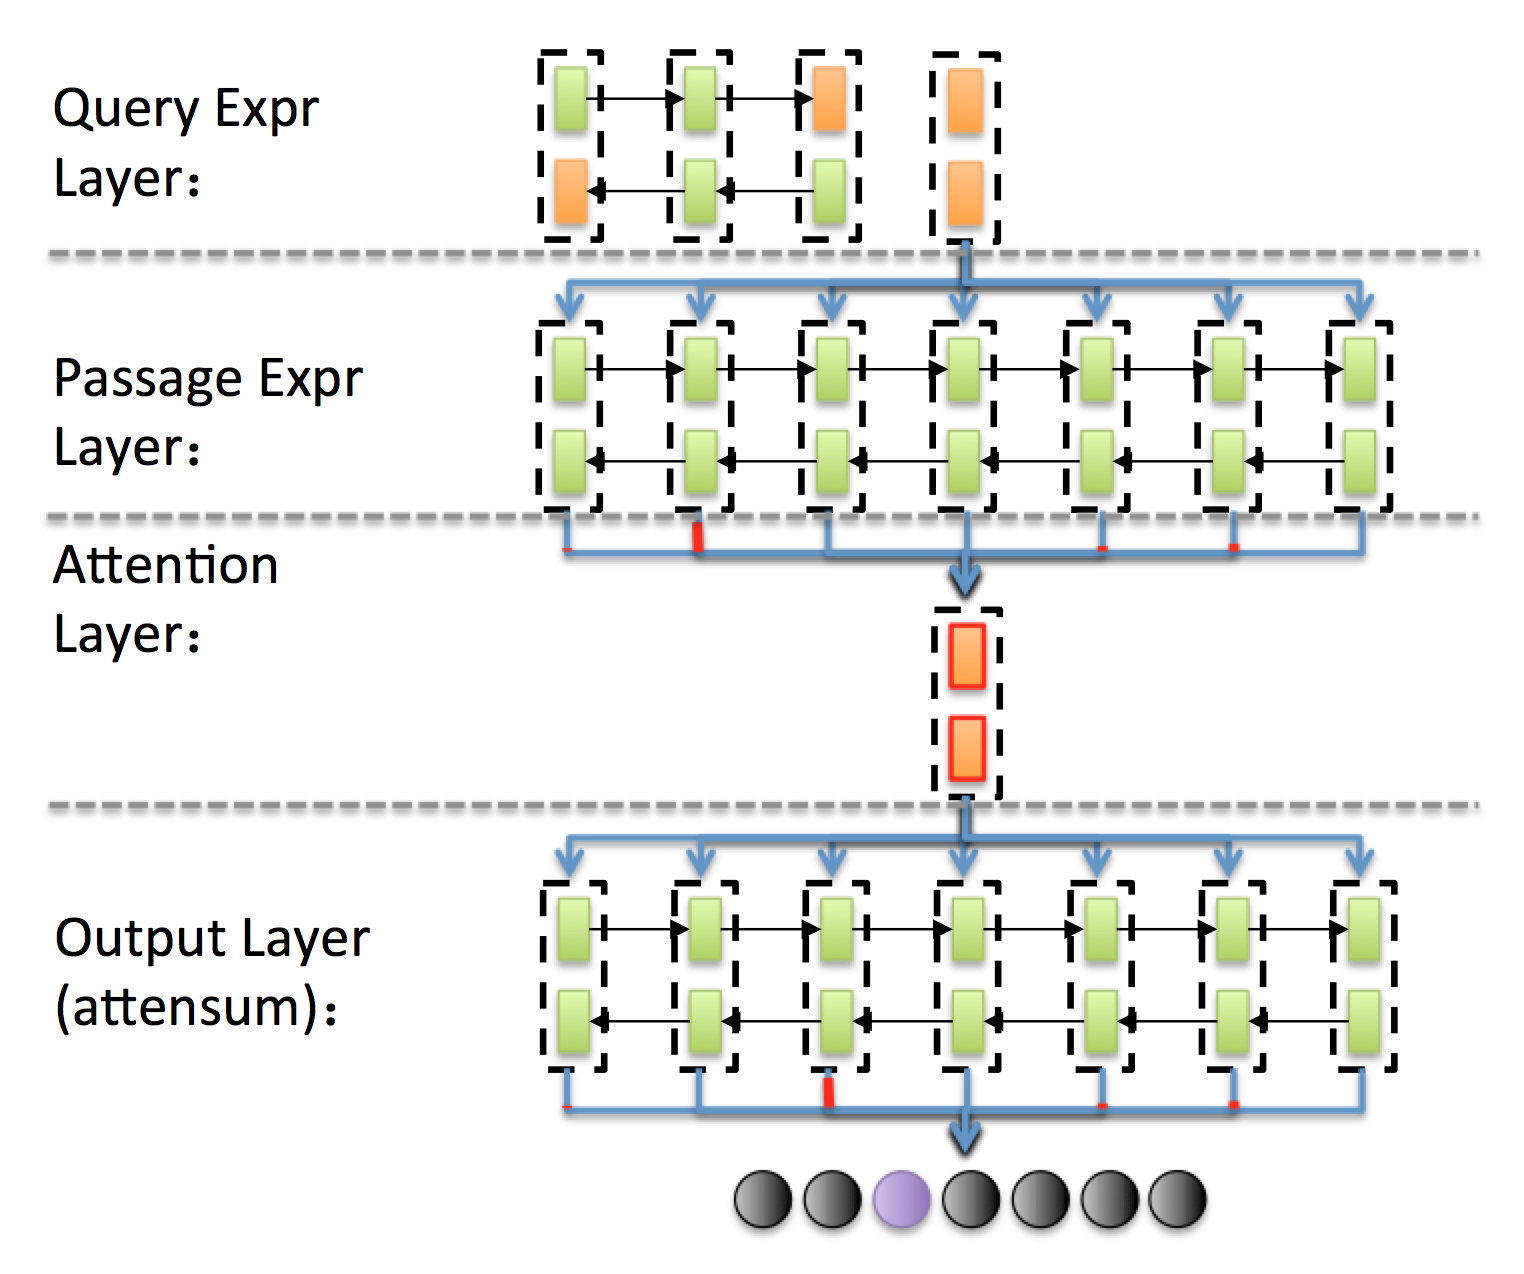
\includegraphics[width=80mm]{picture/attention_attensum.PNG}
	\caption{Attention-Attensum Reader。同Attention Reader相比,仅仅在输出层有所不同。Attentive Reader为每个@entity符号赋予一个特定的权重向量(不同文本中即使@entity所代表的词已经完全不同了,仍旧使用同一个权重向量),而Attention-Attentive Reader的每个@entity的权重向量则是该词在RNN中对应时刻的隐层状态。相比较而言,Attention-Attentive Reader中的权重向量选取更合理。}
	\label{fig:3}
\end{center}
\end{figure}

\begin{enumerate}
    \item {\bf 动机}:@entity实体在不同文章中表示不同的词,而在softmax解码的时候,一个@entity符号对应唯一的权重向量,这就使得attention reader在解码的时候实际上是“混乱”的,至少这加大了训练的难度;
    \item  {\bf 做法}: 需要的其实就是为每个@entity符号寻找一个对应的有实际意义的权重向量,那么可以直接使用RNN编码过程中@entity符号对应时刻的隐层状态作为权重向量。
    \item  {\bf  目前状态}:截至目前,已经尝试运行三次,均因服务器故障以及资源问题等原因未能获得顺利运行;
    \item  {\bf  结论以及后续}:继续做;但是在写作本文的时候,发觉一个潜在的问题,就是抛开所谓attention,softmax,权重向量、隐层状态等等概念,实际上从数学角度而言attention layer同output layer在做同一件事情,做两次同样的事情是否是有意义的?当然另外一角度也说明这个模型本身非常便于扩展叠加多层。
\end{enumerate}

\section{log\_linear系列实验}
\subsection{Baseline}
Baseline采用八种特征,包括候选实体是否出现在文章中、出现在问句中、频率、第一次出现在文章中的位置、n-gram特征、依存特征等等。Chen的文章报出来的结果是67.1\%,我这边实现出来的结果是65.8\%。训练使用开源的lambdaMART。
\subsection{增加NN输出结果为新特征的实验}
\subsubsection{lambdaMART}
将NN给每个候选词打的分数作为特征添加到lambdaMART,做了两组实验,第一组是直接将分数(概率)作为特征;第二组是将NN给出的概率最高的那个词设置特征为1其余为0;两组实验均没有达到65.8\%,感觉不太对,于是换成SVM再做一下。
\subsubsection{SVM}
直接使用libsvm训练,单机器一直没有训练出来结果,训练一个礼拜未果,放弃;

\noindent 使用线性核的rankSVM来训练,性能是62\%,但是奇怪的是如果使用开发集作为训练数据却可以获得68\%的效果;

\noindent 非线性核的rankSVM也没有跑出来;

\noindent 使用公司的LTR来做,gbrank效果是67\%。

\noindent 之后没有继续该方向的实验。


\section{NN框架下融入经典特征的系列实验}
\subsection{Attentive Reader}
\subsubsection{Baseline}
Figure~\ref{fig:1} 是经典的Attentive Reader模型框架图。从最开始的调研到初步实现,再到调参,性能只能抵达65\%,在陈丹琦公布源码之后,找到其中诸多trick,之后baseline性能抵达72.6\%,同丹琦报出来的结果基本持平。

这一部分的总结是:网络的维度、embedding的维度以及数据预处理,对于性能影响最大,而其他超参基本上没有本质影响。调参的时候太过谨慎,每次只调一个,造成时间和计算资源的低效率使用。
\subsubsection{经典特征丰富模型输入}
\begin{enumerate}
    \item {\bf 动机}:做负例数据分析的过程中,一方面发现部分情况下(25\%)目标词并没有被很好的刻画,比如目标词分明是个人、或者是机构,而返回的答案却是个“山”、在这种情况下,借助经典特征来帮助Reader“刻画”目标词便成了一个可行的方向。
    \item  {\bf 做法}: 提取依存关系的类型作为特征,加入到输入层,也即输入到RNN中的是词向量和对于特征向量的拼接。依存关系是有方向的,根据提取入边或者出边的关系类型作为特征分别作了一组实验;此外,将依存关系中父节点的词作为特征以及postag作为特征,也分别做了一组实验;上述四组实验均采用直接拼接的方法,一次对应,做了四组词向量和特征向量过一个非线性层预处理的实验;
    \item  {\bf  结果}:由于做的时候是为了做ensemble,所以没有对单独的模型做特别的调参,就综合效果而言,加入依存关系类型的实验效果在69\%左右,加入依存父节点词作为特征的实验效果在71\%,计入postag性能在70\%,而非线性并没有对性能造成明显影响;
    \item  {\bf  猜想}:一方面可能是因为特征对于任务作用有限,而这八组实验均没有超过baseline(即使没有严格调参这也能说明问题了);另一方面是任务本身的问题,@entity在不同文章中表示不同的内容,这直接导致词向量、对应时刻RNN隐层状态以及解码矩阵中的权重向量,均失去明确的意义,为任务带来混乱。
\end{enumerate}

\subsubsection{经典特征用于调整attention机制}
\begin{enumerate}
    \item  {\bf 动机}:同上一节。
    \item  {\bf 做法}:Attentiive Reader 中Attention层,取query表示和文章中各个时候的隐层状态做点乘,然后softmax获得“权重”。将特征在这个层面直接加入,query表示向量拼接一个目标词的特征向量,而文章各个时刻的隐层状态也拼接各自时刻的词语特征向量,如此直接利用特征干预筛选过程。具体做法上,有三种,其一,仅用01标识出entity的位置,这样便于权重集中到@entity等有效候选实体上面;其二,文章中仅仅@entity具有特征,其他普通词的特征向量全部置为UNK;其三,文章中各个词义均有特征向量。特征向量用的是依存关系中父节点位置上的词。
    \item  {\bf  结果}:由于代码bug,双向rnn返回的隐层状态是反向的,这对于上一节的做法么有影响,却对于本节的做法直接干扰,进而训练所得结果均是没有提升;调整bug之后,attentive reader出现NAN问题,原因不明;由此此时已经调试完成Attensum Reader,而且训练速度更快性能相当,所以转到attensum reader上做实验了,本节实验暂停。
\end{enumerate}

\subsection{Attensum Reader}
\subsubsection{Baseline}
Figure~\ref{fig:2} 是经典的Attensum Reader模型框架图。直接利用attention过程中的权重作为词输出的概率,唯一的不同是需要将同一个词对应的权重加和作为最终该词的概率。baseline效果是72.5\%,而如果使用数据预处理将所有答案全部替换为@entity0,则出现99\%的效果。
\subsubsection{经典特征丰富模型输入}
暂时没有做,鉴于Attention Reader的实验,这一部分暂缓。
\subsubsection{经典特征用于调整attention机制}
\begin{enumerate}
    \item  {\bf  初始attensum}:
        \subitem  {\bf  baseline}:72.65\%;高峰抵达73\%;同时观测到500句左右,集中到entity的概率不足0.5。
        \subitem  {\bf  baseline+仅有entity上有特征其他词语特征为UNK}:72\%;同baseline一样,500多句集中到entity的概率不足0.5	去掉针对特征embedding的L2正则之后,性能没有提升,有300多句集中到entity的概率不足0.5。
        \subitem  {\bf  baseline+所有词语均有特征}:72.1\%;同baseline一样,500多句集中到entity的概率不足0.5。
        \subitem  {\bf  baseline+entity用特征1标示其他词语用0标示}:72.3\%;仅用01表示entity位置,去掉针对embedding的L2正则,优化损失函数(鼓励概率集中到entity上)	全部句子集中到entity;再度优化之后,性能徘徊在72.5\%左右。
    \item  {\bf  改变TF输入方式以及去掉损失优化以及仅在entity上面解码}:
        \subitem  {\bf  baseline+仅有entity上有特征其他词语特征为UNK}:70\%;
        \subitem  {\bf  baseline+所有词语均有特征}:正在做;
        \subitem  {\bf  baseline+entity用特征1标示其他词语用0标示}:等待做;
        \subitem  {\bf  baseline+特征选取Postag}:等待做;
\end{enumerate}

\subsection{基于经典特征做Rerank的实验}
\begin{enumerate}
    \item  {\bf  动机}:利用特征来帮助选择,同前面两节将特征融入NN的做法不同,这边是基于NN给出候选答案,然后基于特征在候选答案中进一步筛选。
    \item  {\bf  做法}:利用多种NN模型,attentive reader、attentive reader+经典特征丰富,共计五种模型,然后每个模型随机选择两个中间结果(性能已经稳定),这样每个文本-问句对共有十个候选答案。一般而言,这十个候选答案中只有两三个不同的@entity;利用目标词的特征向量和这些候选词的特征向量点乘,算的权重,权重最大的那个候选答案成为最终的结果。
    \item  {\bf  结果}:性能抵达71\%;而实际上,如果仅仅利用这十个候选答案进行投票,则性能抵达75\%(此处还出过一个比较严重的乌龙事件,前后占用十天时间)。
    \item  {\bf  目前状态}:如此简单的二次筛选就能取得不错的结果,但是接下来怎么做就没有具体规划了。如何更合理的利用经典特征,这是个开放问题。
\end{enumerate}

\section{当前实验总结}
总体而言,将经典特征整合进NN的实验,有两种方式。其一是丰富输入特征,在attentive Reader中并没有取得很好的效果,在Attensum Reader中暂时没有做。其二是将特征用于调整attention机制,之前在Attentive Reader中的实验由于bug导致之前的结果丧失意义,而调整之后的代码出现NAN,于是暂停去做Attensum Reader的对应实验;Attensum Reader的baseline性能正常,在72.5\%左右,而其他已经完成的实验均没有明显突破。

\section{下一步实验计划}
1、 迁移到lego,实验室的机器饱和,速度缓慢。

\noindent 2、 需要做的实验是{\bf 将特征用于调整attention机制}下Attensum Reader的剩余实验 以及  Attentive的实验。此外,Attentio\_Attensum Reader的实验也要继续。

\noindent 3、 考虑更换数据集,目前的数据集收到@entity这种没有固定语义的现象影响严重,各种模型均受此影响。
 
\end{document}
